\documentclass[]{article}
\usepackage[utf8]{inputenc}
\usepackage{verbatim}
\usepackage{tikz}
\usetikzlibrary{automata, positioning, arrows}
%opening
\title{Practicum \#3 bis\\}
\author{Horacio G\'omez-Acevedo, PhD\\
	Department of Biomedical Informatics\\
	UAMS}


\begin{document}

%\maketitle



\begin{figure}[ht]
	\centering
	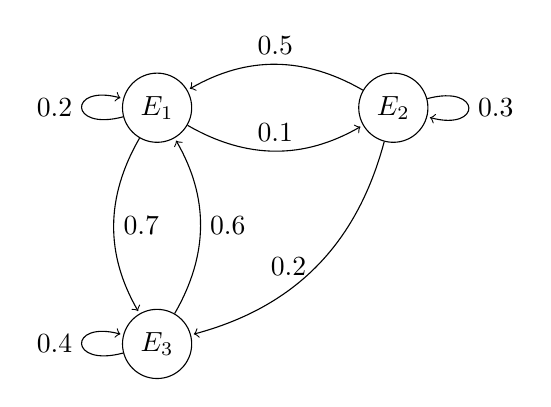
\begin{tikzpicture}[->,shorten >=1pt, node distance=3cm,auto]
%	\node[state, initial] (1) {$q_1$};
	\node[state] (1) {$E_1$};
	\node[state, right of=1] (2) {$E_2$};
	\node[state, below of=1] (3) {$E_3$};
	\draw (1) edge[above,bend right] node{0.1} (2)
	(2) edge[above,bend right] node{0.5} (1)
	(1) edge[loop left] node{0.2} (2)
	(1) edge[right, bend right] node{0.7}(3)
	(3) edge[right, bend right] node{0.6}(1)
	(2) edge[left, bend left] node{0.2}(3)
	(2) edge[loop right] node{0.3} (2)
%	(2) edge[loop left] node{0} (2)
%	(2) edge[below] node{1} (4)
%	(1) edge[above, bend right, right=0.3] node{1} (4)
%	(4) edge[above, bend right, right=0.3] node{1} (1)
%	(4) edge[right] node{0} (3)
	(3) edge[loop left] node{0.4} (3);
	\end{tikzpicture}
	\caption{Markov chain  $H_2$}
\end{figure}

\end{document}